\part{Ontwerp}
\label{ontwerp}

%
% Systeemmodel
%

\chapter{Systeemmodel}
\label{ontwerp:systeemmodel}

De eerste stap van het ontwerp was de identificatie van de verschillende deelsystemen, en op welke toestellen die te vinden zijn. Hiertoe hebben we eerst gekeken naar de verschillende taken die het systeem als een geheel moet vervullen. Zo moet het systeem:
\begin{itemize}
\item Voorstellingen weergeven, en gebruikersinvoer verwerken;
\item Toelaten om eenvoudig voorstellingen te wijzigen, zonder veel technische bagage;
\item Voorzien in een gebruiksvriendelijke beheersinterface;
\item Dit alles voldoende robuust uitvoeren.
\end{itemize}

Hiermee konden we de verschillende deelsystemen identificeren. Zo zijn er natuurlijk de kiosken, die instaan voor de weergave van de voorstellingen, en de verwerking van gebruikersinvoer. Om het systeem flexibel te houden, zullen we de kiosken zo inrichten dat zowel de configuratie als de weer te geven voorstellingen zich niet op voorhand op de kiosk bevinden, maar van een centrale server gehaald worden. Diezelfde centrale server kan dan ook voorzien in een beheersinterface, waarbij de status van de verschillende kiosken gevisualiseerd wordt, en de administrator eventueel bepaalde acties kan ondernemen. Al deze functionaliteit zullen we bundelen binnen het specifiek hiervoor ontworpen applicatie-raamwerk, waarvoor we ook een communicatieprotocol zullen voor moeten definiëren.

\begin{figure}
	\includegraphics[width=\textwidth]{diagrammen/ontplooiingsdiagram}
	\caption{Ontplooiingsdiagram}
\end{figure}

In de volgende hoofdstukken zullen we nu elk van deze deelsystemen, en al wat daar bij hoort, tot in details uitwerken. Zo zullen we ook frequent bestaande technologieën hergebruiken, of net een gerichte keuze maken zodat hergebruik mogelijk wordt. Daarbij gaan we meestal uit van een initiële selectie aan technologieën die gebruikt kan worden om een specifiek doel te bekomen, waarna de selectie uitgedund wordt tot er slechts 1 mogelijkheid overblijft. Het valt op te merken dat we bij dergelijke selectieprocedures steeds een impliciete doch sterke voorkeur zullen stellen voor open technologieën, waarvoor er een gratis, cross-platform en open-source implementatie bestaat. Dat we kiezen voor technologieën met een kosteloze implementatie, vloeit voort uit het beperkte budget dat toegekend is door de MIRA vzw. Het cross-platform aspect is belangrijk omdat op termijn de applicatie misschien op een ander systeem zal moeten draaien, alsook het interessant zou zijn om indien het product succesvol blijkt, het open te stellen voor andere bedrijven. Het open-source kenmerk tenslotte kent zijn oorsprong weliswaar deels in idealistische gronden, maar blijkt in de praktijk ook zeer praktisch te zijn. Zo is het tijdens de realisatie van het project verschillende keren extreem nuttig gebleken om vrije toegang te hebben tot de broncode van de bibliotheek.


%
% Applicatie
%

\chapter{Applicatie}
\label{ontwerp:applicatie}

Het volgende hoofdstuk zal het ontwerp van de applicatie bespreken. Daarbij zullen we eerst de technologieën vastleggen, om vervolgens het exacte gebruik ervan te documenteren. In realiteit was dit proces echter niet zo afgelijnd: vaak leidde een bepaalde beslissing tot het terugkomen op een voorheen gemaakte keuze. In meerdere gevallen zal het dan ook voorkomen dat een specifieke eis uit het niets gegrepen lijkt, of bevooroordeeld schijnt te zijn. Toch is dit niet het geval, pas na afloop van het hoofdstuk zal het totale plaatje duidelijk worden, nadat alle beslissingen mooi in hun voegen gevallen zijn.

\section{Voorstellingen}
\label{ontwerp:applicatie:voorstellingen}

\subsection{Formaat}

Aan het formaat van de voorstellingen worden een aantal specifieke eisen gesteld:
\begin{itemize}
\item Efficiënt te distribueren over het netwerk;
\item Flexibel en toekomstgericht;
\item Terugwaarts compatibel met de huidige voorstellingen;
\item Laagdrempelig.
\end{itemize}

Zoals reeds gezegd bevinden de oude voorstellingen zich op een Dvd-schijf, in videoformaat. Het nieuwe formaat moet dus in staat zijn om video's weer te geven, eventueel na bepaalde conversies.

Na verschillende formaten vergeleken te hebben, hebben we besloten gebruik te maken van een combinatie van \ac{html} en Javascript. Die combinatie wordt vaak op het web gebruikt voor het maken van websites, en laat toe om heel dynamische voorstellingen te ontwerpen. Ook is het mogelijk om, zonder enige aanpassing aan het omliggende raamwerk, gebruik te maken van extra Javascript bibliotheken, waardoor de mogelijkheden onbegrensd zijn.

Hoewel de complexiteit enorm lijkt, zal de weergave van dergelijke voorstellingen nog relatief eenvoudig kunnen gerealiseerd worden, dit omdat \ac{html} en Javascript al jarenlang weergegeven worden binnen webbrowsers. We zullen dus de vruchten kunnen plukken van decennia aan ontwikkeling, door gebruik te maken van de \emph{rendering engines} uit verschillende browsers.

Sinds de nieuwste versie van de \ac{html} standaard, versie 5, is er ook voorzien in een \texttt{<video>} tag, die toelaat om videofragmenten weer te geven. Hierdoor voldoen we ook aan de vereiste terugwaartse compatibiliteit, al is het met enige beperkingen. Momenteel is het immers nog niet duidelijk welke videostandaard algemeen zal ondersteund worden in de \texttt{<video>} tag, meer nog, er woedt een hele strijd tussen de verschillende fabrikanten en ontwikkelaars. Afhankelijk van welke versie van welke rendering engine we gebruiken, zullen we moeten kiezen uit een andere verzameling videostandaarden.

Ook efficiënte netwerktransmissie wordt bekomen door gebruik te maken van HTML en Javascript. Alle code wordt immers opgeslagen in tekstformaat, en de videostandaarden (los van welke we uiteindelijk zullen gebruiken) zijn steeds geselecteerd wegens hun nut in context van webpagina's, waar efficiënte compressie al even belangrijk is. Wanneer men een nieuwe voorstelling ontwerpt, kan men door gebruik te maken van de vele mogelijkheden die \ac{html} versie 5 biedt, de netwerkbelasting helemaal minimaliseren. Hiertoe kunnen bijvoorbeeld binaire afbeeldingen vervangen worden door vectorafbeeldingen, en scripted animaties verkozen worden boven ordinaire videofragmenten.

Tenslotte is dit formaat voor de voorstellingen ook vrij laagdrempelig. Veel mensen hebben een basiskennis over HTML, en indien ze dit niet hebben is het eenvoudig te leren via de overvloed aan tutorials die er beschikbaar zijn. Ook is er geen nood aan een speciale \emph{toolchain}: zowel \ac{html} als Javascript bronbestanden kunnen gewijzigd worden in elke tekstverwerker, het resultaat kan eenvoudig gecontroleerd worden in een lokaal geïnstalleerde browser, en compilatie is al helemaal overbodig.
Een mogelijk probleem is de beperkte scheiding tussen design en logica: wanneer dynamiek vereist is, moet de ontwerper nogal snel enige kennis hebben van Javascript. Toch kan dit verholpen worden door gebruik te maken van \ac{wysiwyg} editors, al moet het gezegd worden dat die anno 2011 nog niet zo goed gebruik maken van alle mogelijkheden die deze nieuwe standaard biedt.

\subsection{Repository}

Zoals hierboven reeds vermeld, zullen noch de nieuwste voorstellingen noch de configuratie zich direct op de relevante kiosken bevinden, maar dynamisch van de centrale server gedownload worden. Indien voorzien wordt in een gebruiksvriendelijk systeem om de presentaties te wijzigen, maakt dit het leven van de administrator ook een pak gemakkelijker nu hij niet meer moet deployen naar elke kiosk apart.

Initieel zijn we op zoek gegaan naar een \strong{database-systeem} om dit te implementeren. Hoewel dergelijke systemen vooral sterk zijn in het herbergen van gestructureerde data, zou het perfect mogelijk zijn om er de eerder bestandsgeoriënteerde voorstellingen in op te slaan. Efficiënte overdracht wordt echter niet voorzien, alsook zou het vrij moeilijk zijn om een gebruiksvriendelijke interface te bouwen bovenop dit systeem.

Een andere verzameling technologieën die we overwogen hebben, waren de \strong{Enterprise Content Management} systemen. Hierbij vinden we al vaker een geïntegreerde beheersinterface, alsook komt het frequent voor dat een reeds aanwezig versiebeheer-systeem zorgt voor efficiënte dataoverdracht. Toch voldeed deze oplossing niet, daar bij dergelijke systemen de nadruk vaak nog explicieter ligt op gestructureerde data, waardoor het niet praktisch zou zijn om er onze ongestructureerde voorstellingen in op te slaan.

Daarom hebben we uiteindelijk te stap gemaakt naar gedediceerde \strong{versiebeheer-systemen}. Hierbij is efficiënte overdracht van gegevens een basiseigenschap, alsook zorgt het bestandsgeoriënteerde aspect voor een relatief gebruiksvriendelijke interface. Zo kan een administrator heel gemakkelijk lokaal enkele wijzigingen doorvoeren aan een voorstelling, het resultaat testen in zijn browser, en indien gewenst zijn werk doorsturen naar de centrale server.

Maar er bestaan tientallen versiebeheersystemen, die we elk gepeild hebben aan ons eisenpakket:
\begin{itemize}
\item Client-server georiënteerd;
\item Efficiënte omgang met binaire bestanden.
\end{itemize}

Gezien de uiteindelijke keuze van het applicatieprotocol (zie onderdeel \ref{ontwerp:applicatie:applicatieprotocol}), komen hier nog twee eisen bij:
\begin{itemize}
\item Beveiliging via \ac{ssl};
\item Te gebruiken over \ac{http}.
\end{itemize}

Er zijn maar weinig versiebeheersystemen die aan dit eisenpakket voldoen. Meer nog, na een uitgebreide vergelijking, blijkt enkel \ac{svn} een geschikte keuze te zijn. Voor \ac{svn} bestaan er tevens Java-bindings, te vinden in de \makeurl{http://code.google.com/p/svnj/}{SVN-J} bibliotheek, waardoor de repository als 1 geheel zou kunnen geïntegreerd worden met de rest van de serverapplicatie. Jammer genoeg is de bibliotheek echter niet matuur genoeg, waardoor we zullen moeten gebruik maken van een overkoepelende webserver zoals Apache. Hierdoor wordt de binding tussen de applicatie en de repository iets minder sterk (wat bijvoorbeeld extra configuratie zal vereisen), maar het is de trade-off nodig om een realistisch systeem te bekomen.

\subsection{Repository layout}

Hoewel het nu bepaald is dat we een bestandsgeoriënteerde \ac{svn}-repository zullen gebruiken, ligt de exacte layout van de bestanden daarin nog niet vast. Aangezien zowel de voorstellingen als de kioskconfiguratie erin zal moeten opgeslagen worden, is het belangrijk om op voorhand een eenduidige structuur vast te leggen die tevens toelaat om eenvoudig wijzigingen te detecteren.

\begin{codefragment}
\begin{verbatim}
+-repository/
  |
  +-configurations/
  | |
  | +-hires.ini
  | |
  | +-nosound.ini
  |
  +-presentations/
  | |
  | +-presentation1/
  |   |
  |   +-config.ini
  |   |
  |   +-index.html
  |
  +-kiosks/
    |
    +-kiosk1.ini
\end{verbatim}
\caption{Voorbeeld van een repository layout.}
\end{codefragment}

Op het hoogste niveau zal de repository bestaan uit drie mappen. In de \texttt{configurations} map bevinden zich bestanden die een configuratie typeren, elk uniek geïdentificeerd door hun bestandsnaam. De configuratie bepaalt volledig hoe een kiosk zich zal gedragen. Zo wordt er voorzien in configuratiesecties voor de weergave, het geluid, het netwerk, enzovoort. Ook kan een configuratie specificeren welke voorstelling moet weergegeven worden, maar die informatie zal zich meestal bevinden in de kiosk-specifieke configuratiebstanden in de \texttt{kiosks} map. Daarin bevindt er zich een configuratiebestand per kiosk, waarin opnieuw de kiosk volledig kan geconfigureerd worden. Elk configuratiebestand (hetzij in de \texttt{kiosks} map, hetzij in de \texttt{configurations} map) kan ook specificeren welke andere configuraties tegelijk moeten ingeladen worden, waardoor gemeenschappelijke instellingen kunnen geabstraheerd worden.

De \texttt{presentations} map tenslotte bevat de effectieve voorstellingen, elk in een aparte map. In die map bevinden zich de bestanden nodig om de voorstelling weer te geven, alsook een configuratiebestand dat nu enkel specifieke eigenschappen van de presentatie configureert.

\begin{codefragment}
\begin{verbatim}
[configuration]
description=Configuration for kiosk1.
load=nosound;hires

[presentation]
name=presentation1
\end{verbatim}
\caption{Voorbeeld van een kiosk configuratiebstand, \texttt{kiosks/kiosk1.ini}.}
\end{codefragment}

\begin{codefragment}
\begin{verbatim}
[configuration]
description=Configuration for kiosks without sound.

[sound]
volume=0
\end{verbatim}
\caption{Voorbeeld van een gedeeld configuratiebestand, \texttt{configurations/nosound.ini}.}
\end{codefragment}

\begin{codefragment}
\begin{verbatim}
description=Sample presentation 1.
landing_page=index.html
\end{verbatim}
\caption{Voorbeeld van een voorstelling configuratiebestand, \texttt{presentations/presentation1/config.ini}.}
\end{codefragment}

\section{Applicatieprotocol}
\label{ontwerp:applicatie:applicatieprotocol}

Het applicatieprotocol zorgt voor de communicatie tussen de verschillende componenten. Omdat dit protocol instaat voor verschillende taken, zullen we dan ook gebruik maken van verschillende protocollen, elk meest geschikt voor de taak die ze moeten realiseren.

Omdat we er naar streven om geen configuratie te voorzien op de kiosken, zal een kiosk na aanmelding op 1 of andere manier moeten geconfigureerd worden. We kiezen ervoor om die configuratie uit te laten gaan van de server, die via een \strong{remote procedure protocol} de nodige configuratiemethodes op de kiosk aanroept. Hiertoe moet bij aanmelding van een kiosk, de server een bericht krijgen, wat we kunnen realiseren met een \textbf{service discovery protocol}. Vervolgens moet de kiosk, na geconfigureerd te zijn, de data kunnen ophalen van de centrale server. De locatie van die data is doorgespeeld als onderdeel van de communicatie, en kan opgehaald worden via het \textbf{dataprotocol}.

\subsection{Beveiliging}

Ook is het vanuit bedrijfsperspectief steeds interessant om bepaalde methodes van beveiliging te overwegen. Encryptie is niet belangrijk, daar geen van de verzonden data gevoelige informatie blootgeeft. Een vorm van authenticatie is echter wel interessant, om te voorkomen dat een kwaadwillende derde de configuratie op een kiosk vervalst, of verkeerde voorstellingen verdeelt. Voor het service discovery gedeelte zal blijken dat authenticatie minder belangrijk alsook moeilijk te implementeren is (het netwerk kan hoogstens vertraagd of licht verstoord worden, corruptie van gegevens is onmogelijk).

De overige twee protocollen willen we natuurlijk op een uniforme manier van authenticatie kunnen voorzien. Hiertoe is het interessant om gebruik te maken van \ac{ssl}, een populair en veilig beveiligingsmechanisme. Bovendien kunnen we, indien beide protocollen gebruik maken van \ac{http} transport, het beveiligingsaspect louter in de overkoepelende webserver implementeren, zodat de deelprotocollen zelf geen \ac{ssl} moeten implementeren, maar toch beveiligd zijn door een robuust authenticatiemechanisme. Enkel voor clientside gebruik (zoals bij de applicatieserver, die contact moet kunnen opnemen met een XML-RPC interface op de kiosken) zal er specifieke configuratie nodig zijn om \ac{ssl} te kunnen toepassen.

\subsection{Service discovery}

Service discovery is een onderdeel van de "Zeroconf" standaard, een verzameling technieken die instaat voor het initialiseren van een netwerk zonder daarbij te voorzien in expliciete configuratie. Service discovery staat daarbij in voor het ontdekken van andere toestellen, alsook eventuele services die erop aanwezig zijn. Meestal voorzien dergelijke protocollen in twee elementaire features: het \emph{publishen} van services, waarbij een toestel te kennen geeft wat zijn mogelijkheden zijn, en het \emph{browsen} van services, waarbij een toestel actief of passief op zoek gaat naar bepaalde services binnen het netwerk.

In de context van dit systeem zal een nieuwe kiosk na het opstarten zijn naam en adres publiceren op het netwerk. Een eventuele server zal passief luisteren naar een dergelijke publicatie, en de informatie daarbij bekomen gebruiken om over te gaan tot configuratie van de kiosk in kwestie.

Opnieuw bestaan er verschillende technologieën die voorzien in deze elementaire functionaliteit. Om een selectie te kunnen maken, stellen we enkele bijkomende eisen: 
\begin{itemize}
\item Vereist geen extra infrastructuur;
\item Cross-language implementatie;
\item Eenvoudig te gebruiken.
\end{itemize}

Een veelgebruikt protocol voor service discovery, is het  \strong{\ac{ssdp}}, deel van het \ac{upnp} systeem. Dit door Microsoft-ontwikkeld systeem, biedt een heel uitgebreid en generisch raamwerk voor service discovery, waarbij die services volledig beschreven worden door het \ac{dcp}. Het geheel steunt sterk op XML en SOAP, en is strikt beheerd door het \ac{upnp} Forum. Hoewel het protocol essentieel wel voldoet aan onze eisen, is het groot en log, en biedt het veel te veel mogelijkheden die we toch niet gaan gebruiken.

Een compacter alternatief is \strong{\ac{mdns}}, onderdeel van het door Apple ontwikkelde Zeroconf systeem. Zoals de naam doet vermoeden, is dit een multicast uitbreiding van het \ac{dns}, dat de \texttt{SRV} records gebruikt om services te publiceren. Dit is een veel eleganter systeem, essentieel slechts een eenvoudige uitbreiding van een bestaande technologie, maar kent zo ook zijn tekortkomingen. Zo worden bijvoorbeeld de mogelijkheden van elke service gedetailleerd via een verder niet gespecificeerd tekstveld. Dergelijke tekortkomingen zijn echter niet van belang in de context van dit systeem, waardoor we zullen kiezen voor dit systeem. Bovendien kent mDNS bindings voor zowel Java als Qt, de twee frameworks die we zullen gebruiken bij de effectieve realisatie van de deelsystemen (zie sectie \ref{ontwerp:applicatie:server} en \ref{ontwerp:applicatie:kiosk}).

\subsection{Remote procedure}

Van zodra de server weet heeft van een nieuwe kiosk, moet die overgaan tot de configuratie ervan. Ook moet het mogelijk zijn om acties teweeg te brengen, bijvoorbeeld ten gevolge van acties in de beheersinterface. Daarom zijn we niet op zoek gegaan naar specialistische configuratieprotocollen, maar eerder naar meer generieke \emph{remote procedure} protocollen.

Opnieuw bestaan er vele verschillende remote procedure protocollen, elk met hun specifieke eigenschappen. Grotere enterprise-projecten geven vaak de voorkeur aan technologieën zoals \strong{\ac{soap}} of \textbf{\ac{corba}}, enorme systemen die zeer uitgebreide mogelijkheden kennen. We zullen dergelijke technologieën echter om dezelfde reden vermijden als waarom we \ac{mdns} boven \ac{upnp} verkozen hebben: in de context van dit project is een compacter en eleganter protocol beter te controleren en dus interessanter dan een complex te configureren alleskunner waarbij de meerderheid van de mogelijkheden toch onbenut blijven.

In de categorie van compactere RPC-protocollen vinden we zo bijvoorbeeld \strong{\ac{rest}}. Hoewel dit lichtgewicht, \ac{http}-gebaseerd, en ook veelgebruikt protocol op het eerste zicht aan onze eisen voldoet, kent het zijn mindere kanten. Zo kent het geen eenduidige manier om fouten terug te geven, alsook is het formaat waarin data verstuurd wordt niet gestandaardiseerd. Omdat de implementatie daarvan nog vrij veel werk zou vereisen, besteden we verder geen aandacht aan dit protocol.

De meest courante ontwikkelframeworks zoals .NET en Java kennen meestal ook hun eigen \ac{rpc}-protocol, zoals \strong{.NET Remoting} en \textbf{\ac{rmi}}. Hoewel deze protocollen meestal goed doorontwikkeld en veelzijdig zijn, kunnen ze vaak maar op een enkel platform gebruikt worden en zijn ze al zeker niet cross-language.

Ook hebben we meer moderne \ac{rpc}-frameworks overwogen zoals \strong{Apache Etch}, of \textbf{Apache Thrift}. Deze vrij nieuwe en tevens veelbelovende systemen bleken echter enkele kritieke eisen mis te lopen. Zo kent Apache Etch slechts weinig language bindings, en kent geen van beide een authenticatiemechanisme. Omdat beide verlopen over een eigen protocol, vallen ze ook niet te overkoepelen door een SSL webserver.

Daarom hebben we uiteindelijk gekozen voor \strong{XML-RPC}, een zeer simplistisch \ac{rpc}-protocol dat XML-geformatteerde berichten verstuurd over \ac{http}. Hierdoor wordt het mogelijk om op een transparante manier een vorm van authenticatiecontrole toe te voegen. Toch kent XML-RPC enkele fundamentele problemen, zoals het inefficiënte berichtformaat. Omdat we echter berusten op een apart dataprotocol, is dit geen groot probleem. Ook is de specificatie, om het zacht uit te drukken, vrij beperkt. Dit kan echter een voordeel zijn: de ermee geïmplementeerde interface wordt er compact mee gehouden, en valt eenvoudig te gebruiken vanuit verschillende talen. Dit wordt verder vereenvoudigd door het groot aantal implementaties, voor de meeste talen zijn er verschillende te vinden.

\subsection{Data uitwisseling}

In eerste instantie was het niet de bedoeling gebruik te maken van een derde deelprotocol, maar om de data te versturen over het \ac{rpc} protocol. Na enig onderzoek bleek echter dat zowel het gebruik van een geïntegreerd datasysteem (zie \ref{ontwerp:applicatie:voorstellingen}), als het integreren van een versiebeheersysteem, niet zou lukken.

Nu voorzien we echter in een apart versiebeheersysteem (\ac{svn}), dat vaak gebruikt wordt in combinatie met een webserver. Hierbij wordt het de communicatie bekomen over het \ac{webdav} protocol, dat tevens over \ac{http} getransporteerd wordt. Dit laat ons opnieuw toe op eenvoudige wijze authenticatie toe te voegen, alsook ontlast het ons \ac{rpc} protocol van de effectieve dataoverdracht.

\section{Redundantie en robuustheid}
\label{sec:redundantie}

Een belangrijk aspect van het systeem is dat het robuust is, en dus voorziet in een bepaalde vorm van redundantie. Zoals het hardwareontwerp zal verduidelijken (zie hoofdstuk \ref{ontwerp:hardware}), voorzien we reeds in hardwarematige redundantie onder de vorm van een RAID configuratie. Toch verhelpt dit het fundamentele probleem niet: de centrale server is een \emph{single point of failure}.

Een eerste idee om dit te verhelpen was het voorzien van een \strong{backup server}, die de centrale server continu zou monitoren. In geval van diens falen, zou de failover functionaliteit geactiveerd worden, waarbij de taken van de centrale server integraal overgenomen zouden worden. Gezien het configuratieloze aspect van de opstelling, en het feit dat elk initiatief steeds van de servers uit komt, zou dit totaal geen actie vereisen. Om ervoor te zorgen dat de backup server steeds over de meest recente informatie beschikt, activeert die tevens een (passieve) \ac{mdns} module, alsook registreert die zich bij de primaire server zodat updates aan de presentatie-repository steeds op beide servers aanwezig zijn.
Hoewel deze configuratie zeer elegant lijkt (zeker indien de replicatie alsook promotie/degradatie van de server volledig autonoom verloopt), is ze niet realistisch op budgettair vlak. Het is niet alleen kostelijk om een tweede voldoende krachtige server samen te stellen, maar de aanwezigheid ervan betekent een extra continue energieconsumptie.

Daarom hebben we gekozen voor een tweede piste, namelijk het gebruik van een \strong{backup-cache in de kiosken}. Aangezien embedded hardware vaak komt met een optie voor een kaartslot, is het voordeliger om voor elke kiosk een dergelijke geheugenkaart aan te kopen, en de applicatie te voorzien van de functionaliteit om bij het opvragen van de configuratie en voorstellingen die lokaal op te slaan. Wanneer vervolgens de centrale server onbereikbaar blijkt te zijn, kan steeds gebruik gemaakt worden van deze lokale cache om toch volwaardig te kunnen blijven functioneren.

\section{Server}
\label{ontwerp:applicatie:server}

Zoals reeds vermeld, is de centrale server van essentieel belang in het systeem. Zo verzorgt de server:
\begin{itemize}
\item Configuratie van de kiosken;
\item Opslag en distributie van de voorstellingen.
\end{itemize}

Naast deze elementaire taken, vereenvoudigd de server tevens de werklast van een administrator. We zullen immers voorzien in een beheersinterface die niet alleen een overzicht van het systeem biedt, maar ook toelaat om acties te ondernemen om eventuele problemen te verhelpen.

\subsection{Ontwikkelplatform}

De keuze van het ontwikkelplatform waarvoor we de serverapplicatie zullen ontwikkelen, is van vrij groot belang. Een goede keuze vereenvoudigt en versnelt de ontwikkeling, terwijl een verkeerde keuze tevens de kwaliteit van het eindproduct nadelig kan beïnvloeden.

Opnieuw bestaan er verschillende mogelijkheden die ons essentieel de middelen aanbieden om deze taak te volbrengen. Om een beslissing te kunnen maken, hebben we ons gefocust op de meestgebruikte entiteiten in de wereld van serverapplicaties, namelijk .NET en Java. Hoewel beide kandidaten relatief evenwaardig zijn in de context van deze serverapplicatie, hebben we voor het gemak gekozen voor ontwikkeling in Java. Deze keuze is gemotiveerd door voorgaande ervaringen, maar ook door het feit dat we een voorkeur hebben voor een Linux-gebaseerde omgeving en .NET daar niet goed met samenwerkt.

\subsection{Hergebruik}

\subsubsection{Applicatieprotocol}

Tijdens het ontwerp van het applicatieprotocol hebben we er speciaal op gelet om zoveel mogelijk bestaande technologieën te gebruiken, zodat we net steeds het wiel opnieuw uitvinden alsook tijdens de realisatie zouden gebruik kunnen maken van bestaande kwalitatieve codebibliotheken.

\paragraph{Service discovery} Om de kiosken te kunnen configureren, moet de server kunnen registreren wanneer een nieuw toestel zich aanmeldt. Deze berichten verlopen over \ac{mdns}, wat we in Java kunnen realiseren via de \makeurl{http://jmdns.sourceforge.net/}{JmDNS} bibliotheek. Deze volledig in Java geschreven bibliotheek biedt een volledig platform-onafhankelijke implementatie van het \ac{mdns} protocol, alsook verschillende high-level mogelijkheden om om te gaan met \ac{mdns} berichten.

\paragraph{Remote procedure} De effectieve configuratie wordt gerealiseerd via functieaanroepen, die verlopen over het XML-RPC protocol. Dit is mogelijk via de \makeurl{http://ws.apache.org/xmlrpc/}{Apache ws-xmlrpc} bibliotheek, een zeer uitgebreide en doorontwikkelde bibliotheek voor XML-RPC communicatie.

\paragraph{Data uitwisseling} Opslag en distributie van de voorstellingen zal niet door de applicatie zelf verzorgd worden, maar door een \ac{webdav} toegangspunt die wijst naar een \ac{svn} repository. Hiervoor zijn geen extra voorzieningen in de applicatie vereist. Om de toegang tot zowel de serverapplicatie als de repository op een eenduidige manier te laten verlopen, overkoepelen we beide door een Apache webserver, waardoor de toegang (poortnummer, hostname) op dezelfde manier verloopt, alsook bepaalde instellingen (\ac{ssl}) kunnen weggewerkt worden naar dit hoger niveau.

Hoewel de effectieve dataoverdracht geen voorzieningen in de serverapplicatie vereist, moet er wel een mechanisme zijn dat wijzigingen detecteert en ze kan inladen, om vervolgens eventueel bepaalde kiosken te herconfigureren. Hiervoor hebben we nood aan een client-side \ac{svn} bibliotheek, die ons toelaat gegevens vanuit de repository op te halen en in te laden. Ook moet het mogelijk zijn snel te kijken wat de laatste revisie van de repository is, en om vervolgens op te halen wat er veranderd is sinds de laatste bekende revisie. Met die informatie kan bepaald worden welke configuraties en/of presentaties opnieuw moeten opgehaald worden, om daarna die informatie door te sturen naar de relevante kiosken.
Hoewel er opnieuw verschillende \ac{svn} bibliotheken bestaan, lijkt \makeurl{http://svnkit.com/}{SVNKit} de enige die nog doorontwikkeld wordt. Ook is de bibliotheek geschreven in pure Java, wat opnieuw het geheel platformonafhankelijk maakt.

\subsubsection{Beheersinterface}

Tenslotte moeten we ook voorzien in een beheersinterface. Hiervoor zullen we een servlet-engine gebruiken, zodat we bij het genereren van een webpagina tegelijk toegang hebben tot de hele applicatie. Binnen de Java wereld zijn er verschillende servlet engines, de bekendste wellicht Tomcat en Jetty. Aangezien onze applicatie niet draait rond de webapplicatie, maar dat slechts een deelcomponent is, zullen we niet gebruik kunnen maken van de standaard servlet environment. Door de servlet engine te \emph{embedden} binnen onze applicatie, is het eenvoudiger om tegelijk verschillende andere niet-webgeoriënteerde services actief te hebben (zoals de \ac{mdns} monitor). Zowel Tomcat als Jetty maken het mogelijk om ze te gebruiken binnenin een applicatie, al is het bij de ene al makkelijker dan bij de andere. Er is echter een belangrijk verschil tussen beide: een embedded Tomcat deelt de \ac{jvm} van de applicatie, terwijl Jetty een nieuwe \ac{jvm} opstart. Aangezien we vanuit de servlets toegang willen hebben tot de rest van de applicatie, zonder daar een speciaal communicatieprotocol zoals \ac{rmi} voor te moeten gebruiken, kunnen we enkel Tomcat gebruiken.

Nu de servlet engine vast ligt, moeten we nog bepalen op welke technologie we de servlets zullen bouwen. Om ons niet bezig te moeten houden met hoe de webpagina's gegenereerd worden, zijn we op zoek gegaan naar een widget-oriented framework voor moderne webapplicaties. Zo hebben we uiteindelijk gekozen voor \makeurl{http://vaadin.com/home}{vaadin}, een bibliotheek die toelaat om op een eenvoudige manier met enkel Java code een rijke user-interface te onwerpen. De manier van ontwikkelen leunt nauw aan bij hoe reguliere user-interfaces ontwikkeld worden: event- en widget gebaseerd, zonder zich te moeten bezig houden met het effectief genereren van de interface.

\subsubsection{Logging}

Ook zullen we gebruik maken van het \makeurl{http://logging.apache.org/log4j/1.2/}{Apache log4j} project, om op een uniforme wijze loginformatie te publiceren. Het pakket laat toe om in een extern configuratiebestand te specificeren welke deelmodules hoe gedetailleerd moeten loggen, en wat er met die informatie gedaan moet worden. Zo kunnen we eenvoudig configureren dat kritieke fouten van over heel het systeem moeten doorgemaild worden naar een administrator, of dat een deelsysteem dat nog niet perfect werk zoveel mogelijk informatie moet wegschrijven naar een speciaal logbestand.

\subsection{Structuur}

\textit{Hier komt eventueel nog iets over de structuur van de applicatie.}

\begin{figure}
	\includegraphics[width=\textwidth]{diagrammen/server_structuur}
	\caption{Structuur van de serverapplicatie.}
\end{figure}

\section{Kiosk}
\label{ontwerp:applicatie:kiosk}

Naast de server vormen de kiosken het tweede type toestel in het systeem. Een kiosk staat in voor:
\begin{itemize}
\item Weergave van voorstellingen;
\item Verwerken van gebruikersinvoer.
\end{itemize}

\subsection{Ontwikkelplatform}

De keuze van het ontwikkelplatform is eens te meer belangrijk voor het verloop van de ontwikkeling. Nu liggen de eisen echter anders: het platform moet low-level zijn, weinig afhankelijkheden hebben, en toelaten om performante applicaties te realiseren. Opnieuw beschouwen we enkel platformen die werken in combinatie met Linux-gebaseerde besturingssystemen, maar deze keer is de motivatie erachter anders: de meeste embedded hardware ondersteunt enkel een Linux-distributie. Gezien we het aantal afhankelijkheden ook beperkt willen houden, is een geïnterpreteerde taal niet ideaal.

Het ontwikkelplatform \makeurl{http://qt.nokia.com/}{Qt} voldoet vrijwel perfect aan dit eisenpakket. Het platform wordt gebruikt in combinatie met C++, een gecompileerde taal die zeer performante code toelaat. Qt zorgt er echter voor dat ontwikkeling van high-level applicaties zoals deze niet al te arbeidsintensief wordt in het relatief low-level C++. Zo komt Qt met een waaier aan interessante modules om snel een applicatie te realiseren, alsook breidt het C++ uit met enkele syntactische mogelijkheden die het eenvoudig maken om bepaalde high-level technieken te realiseren. Bovendien is Qt inherent platform-onafhankelijk, waardoor het mogelijk wordt om de applicatie later eventueel te hergebruiken in een andere omgeving. Tenslotte biedt Qt ook een \emph{embedded mode}, waarin het zelf voorziet in een windowing system. Hierdoor worden enkele zware afhankelijkheden (zoals X11) vermeden.

\subsection{Hergebruik}

\subsubsection{Applicatieprotocol}

Net zoals dit bij de serverapplicatie het geval was, kunnen we door de nauwgezette selectie van protocollen optimaal gebruik maken van bestaande bibliotheken.

\paragraph{Service discovery} Om de kiosk zichzelf te laten aanmelden in het netwerk, zullen we de \makeurl{http://avahi.org/}{Avahi} imlementatie van het \ac{mdns} protocol gebruiken. Deze relatief platform-onafhankelijke bibliotheek komt standaard met Qt4-bindings, die echter niet zo gebruiksvriendelijk zijn en lijken sterk op de oorspronkelijke C bibliotheek. Gelukkig hebben we als onderdeel van het \makeurl{http://gitorious.org/qtmediahub}{QtMediaHub} project een \makeurl{http://gitorious.org/qtmediahub/qtmediahub/trees/master/src/3rdparty/libqavahi}{wrapper} voor de standaard Avahi Qt4-bindings gevonden, die op zeer gebruiksvriendelijke manier (gebruik makende van typische Qt paradigma) toelaat om te interfacen met de Avahi bibliotheek.

\paragraph{Remote procedure} Hiervoor moet de kiosk een XML-RPC server implementeren, waarvoor op zijn beurt een \ac{http}-server nodig is. Hoewel het niet veel werk zou zijn om zelf een eenvoudige server te implementeren (met dank aan de vele hulpmiddelen die Qt biedt), kiezen we er voor om gebruik te maken van een bestaande bibliotheek: \makeurl{http://code.google.com/p/qtxmlrpc/}{QtXmlRpc}. Deze bibliotheek, waarvan de code al vrij goed getest is, komt met een simpele \ac{http}-server die toch ondersteuning biedt voor SSL communicatie.

\paragraph{Data uitwisseling} De kiosk moet in staat zijn een \ac{svn} repository te klonen indien de \ac{webdav} locatie ervan doorgespeeld geweest is. Hoewel we dit best zouden kunnen oplossen door gebruik te maken van de \ac{svn} binary, is dit geen platform-onafhankelijke oplossing, die bovendien niet mooi te integreren valt binnen een applicatie. Daarom zijn we op zoek gegaan naar een C++ bibliotheek, liefst specifiek voor het Qt framework, die ons toelaat gegevens van een \ac{svn} repository binnen te halen zonder daarbij te berusten op een lokaal geïnstalleerde \ac{svn} applicatie. Zo zijn we terecht gekomen bij het \makeurl{http://kdesvn.alwins-world.de/}{KDESvn} project, een KDE frontend voor \ac{svn} repositories. We zijn natuurlijk niet geïnteresseerd in die applicatie, maar in de code die het gebruikt om toegang te krijgen tot \ac{svn} repositories. Daartoe heeft het KDESvn project een bibliotheek ontwikkeld, namelijk \makeurl{http://kdesvn.alwins-world.de/browser/trunk/src/svnqt}{svnqt}. Die bibliotheek is vrijwel volledig losgekoppeld van de KDESvn code, wat integratie binnen andere applicaties eenvoudig maakt (hiervan getuige bijvoorbeeld het \makeurl{http://www.anrichter.net/projects/qsvn}{QSvn} project).

\subsubsection{Weergave voorstellingen}

De voorstellingen zijn opgemaakt in een combinatie van \ac{html} en Javascript. Hierdoor kunnen we voor de weergave gebruik maken van de rendering engines ontwikkeld voor verschillende browsers. Zo is er de \makeurl{https://developer.mozilla.org/en/Gecko}{Gecko} rendering engine, ontwikkeld voor gebruik binnen de producten van Mozilla. Ondanks de recente port van Firefox naar het Qt platform, blijft de integratie van Gecko binnen Qt relatief moeilijk.

Daarom zullen we eerder kiezen voor de \makeurl{http://www.webkit.org/}{WebKit} rendering engine, een doorontwikkeling van de KHTML rendering engine. WebKit is een interessantere keuze gezien zijn populaire port naar het Qt framework, \makeurl{http://trac.webkit.org/wiki/QtWebKit}{QtWebKit}. Deze port is een officieel onderdeel van het Qt framework, waardoor het een goed gedocumenteerde en kwalitatief product is.

\subsubsection{Logging}

Net zoals we bij de serverapplicatie gekozen hebben voor een speciale logging bibliotheek onder de vorm van log4j, maken we voor deze applicatie gebruik van het vergelijkbare \makeurl{http://log4qt.sourceforge.net/}{Log4Qt}. Dit is een port van log4j naar het Qt platform, zodat het mogelijk is om op een vergelijkbare manier te voorzien van uniforme logging die nauwgezet kan geconfigureerd worden. Omdat het originele project al enige tijd inactief is, zullen we wel gebruik maken van een meer actief ontwikkelde \makeurl{http://gitorious.org/log4qt}{fork} van Log4Qt. De fork is een doorontwikkeling van het originele project, met enkele bijkomend features en bugfixes.


%
% Hardware
%

\chapter{Hardware}
\label{ontwerp:hardware}

Gezien het beperkte budget is de zoektocht naar gepaste hardware best een uitdaging geweest.

\section{Kiosk}
\label{ontwerp:hardware:kiosk}

Algemeen worden er enkele vrij zware eisen gesteld aan de kioskhardware:
\begin{itemize}
\item Goedkoop: zowel betreffende aankoopprijs, als energieconsumptie;
\item Duurzaam: de hardware moet minstens 5 jaar meegaan;
\item Performant: de applicatie moet vlot werken, alsook een designer toelaten rijke voorstellingen te ontwerpen;
\item Stil.
\end{itemize}

\subsection{Type}

Vooraleer op zoek te gaan naar een specifiek hardwaremodel, is het belangrijk te kiezen wat voor soort hardware we zullen aankopen. Er zijn immers verschillende pistes, elk met hun voor- en nadelen.

\paragraph{Tweedehands thin clients}

Een eerste richting die we verkend hebben, is die van hergebruik. Veel bedrijven hebben in het verleden gebruik gemaakt van thin clients, die wanneer het support-contract verloopt vaak voor een appel en een ei van de hand gedaan worden op populaire tweedehands-sites.

Hoewel dergelijke aanbiedingen wel interessant lijken, biedt een tweedehands thin client te weinig garanties om te gebruiken als hardware voor de kiosken. Zeker betreffende levensduur: een thin client die al vele jaren in werking is kan het steeds na enkele maanden reeds laten afweten, en gezien er geen stabiele bron aan identieke thin clients bestaat vormt dit een reëel probleem. Ook is de hardware extreem beperkt, zo komen thin clients vaak maar met enkele megabytes flash, waardoor de flexibiliteit van het nieuwe voorstellingenformaat snel ongedaan zou gemaakt zijn. Nieuwe thin clients, hoewel aantrekkelijker op hardwaregebied, zijn al helemaal geen optie: de supportcontracten die er altijd mee gepaard gaan duwen de prijs tot onredelijke hoogten, volledig ongeschikt voor de toepassing binnen dit project.

Daarom hebben we besloten om verder geen aandacht meer te besteden aan thin clients, zelfs al zijn die uit prijsoogpunt extreem aantrekkelijk.

\paragraph{Embedded hardware}

Embedded hardware is specifiek ontworpen voor toepassingen als deze. Hoewel vrij prijzig, biedt het daar veel in ruil voor: alle periferie is geïntegreerd op een enkele chip, vaak is er voorzien in specialistische acceleratie-chips, alsook zijn er features te vinden die interessant zijn voor embedded developers (zoals on-board flash, of een SD-kaartslot).

Ook de duurzaamheid is vaak indrukwekkend, mede door het feit dat er enkel solid-state componenten aanwezig zijn. Energieconsumptie is meestal ook een speerpunt, zo verbruikt de Beagleboard slechts 2.2 watt!

\paragraph{Consument-georiënteerde hardware}

Hoewel niet echt geschikt voor dit doel, hebben we ook gekeken naar populaire consument-georiënteerde hardware. In die hardwarecategorie zijn er sinds enkele jaren energie-efficiënte configuraties te vinden, meestal bedoeld voor \ac{nas} toestellen of low-powered computers. Voorbeelden hiervan zijn moederborden gebaseerd op de \makeurl{http://www.intel.com/technology/atom/}{Intel Atom}, of de meer recent geïntroduceerde \makeurl{http://sites.amd.com/us/fusion/apu/Pages/fusion.aspx}{AMD Fusion}. Dergelijke moederborden komen vaak met een geïntegreerde \ac{gpu} (in het geval van de AMD Fusion zit die zelf op de processorchip) en andere periferie, waardoor het moederbord een handig functioneel geheel vormt.

Toch is er ook nood aan extra hardware, waaronder \ac{ram}, een harde schijf, en een voeding. Dat is dan ook direct een nadeel van deze piste: extra componenten verhogen de kans op falen. Andere features die dan wel geïntegreerd zijn op het moederbord, zijn volledig nutteloos voor dit project (zoals een RAID controller, of 5.1 audio).

Ondanks de nood aan die extra hardware blijft de prijs relatief aantrekkelijk. En voor die prijs wordt er meestal vrij veel pure performantie bekomen, wat het gemis aan interessante features deels tegemoet komt. Toch is dit, zeker gecombineerd met de teleurstellende duurzaamheid, niet voldoende om ons er voor te laten kiezen.

\subsection{Model}

Zoals uit de vorige paragraaf blijkt, is embedded hardware de meest geschikte keuze voor dit project. Maar hier eindigt het niet: er bestaan immers verschillende modellen, van verschillende fabrikanten. We zochten naar de volgende features:
\begin{itemize}
\item Aansluitingsmogelijkheden: USB en HDMI;
\item Stereo audio;
\item 100 Mb ethernet;
\item Kaartslot;
\item Flash geheugen (512 MB of meer);
\item Voldoende performant.
\end{itemize}

Zo hebben we gekeken naar de populaire \strong{\makeurl{http://beagleboard.org/}{BeagleBoard}}, een compacte en vrij performante computer, met al de benodigde features en maar weinig meer. De computer komt ook met een speciale \ac{dsp}, alsook een \ac{gpu} die door Qt te gebruiken valt om de performantie te verhogen. Na echter contact opgenomen te hebben met de fabrikant, was die niet geïnteresseerd in de oplage die we zouden bestellen. Het bleek immers dat de BeagleBoard niet bedoeld is voor bedrijven, maar voor beginnende hardware-developers die voor weinig geld willen experimenteren met embedded development.

Daarom zijn we van de BeagleBoard afgestapt, om gelukkig een iets duurder geprijsd maar voor de rest vergelijkbaar product te vinden: de \strong{\makeurl{http://www.igep.es/index.php}{IGEPv2}}. Lange tijd hebben we dan ook gedacht dat dit de uiteindelijke keuze zou worden \textit{(op moment van schrijven is het nog steeds niet helemaal zeker)}. Maar gezien dat iets hogere kostenplaatje, en het feit dat alle extra toebehoren (zoals een voeding, HDMI kabel, omhulsel) nog los moeten aangekocht worden, zijn we toch blijven uitkijken naar een alternatief.

\begin{figure}
	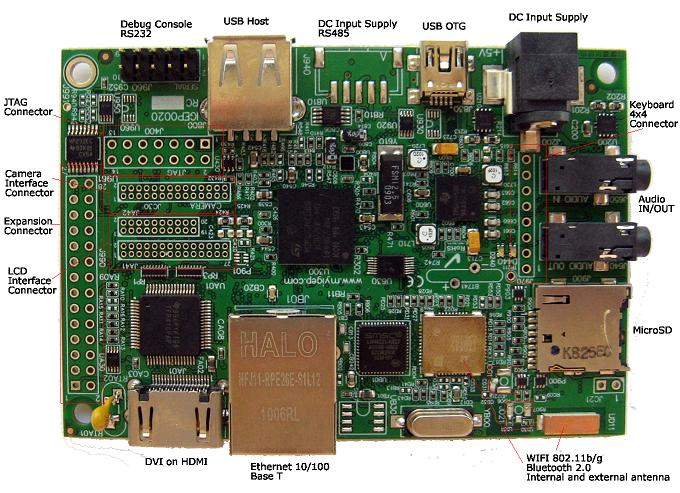
\includegraphics[width=\textwidth]{afbeeldingen/IGEPv2}
	\caption{IGEPv2}
\end{figure}

Dat hebben we gevonden in de vorm van de \strong{\makeurl{http://www.globalscaletechnologies.com/t-guruplugdisplaydetails.aspx}{GuruPlug Display}}. Deze computer is misschien minder krachtig (vooral acceleratiemogelijkheden zijn een prominente afwezige), maar wordt geleverd als een sluitend geheel, waarbij het standaardpakket tevens voorziet van alle nodige kabels.

\begin{figure}
	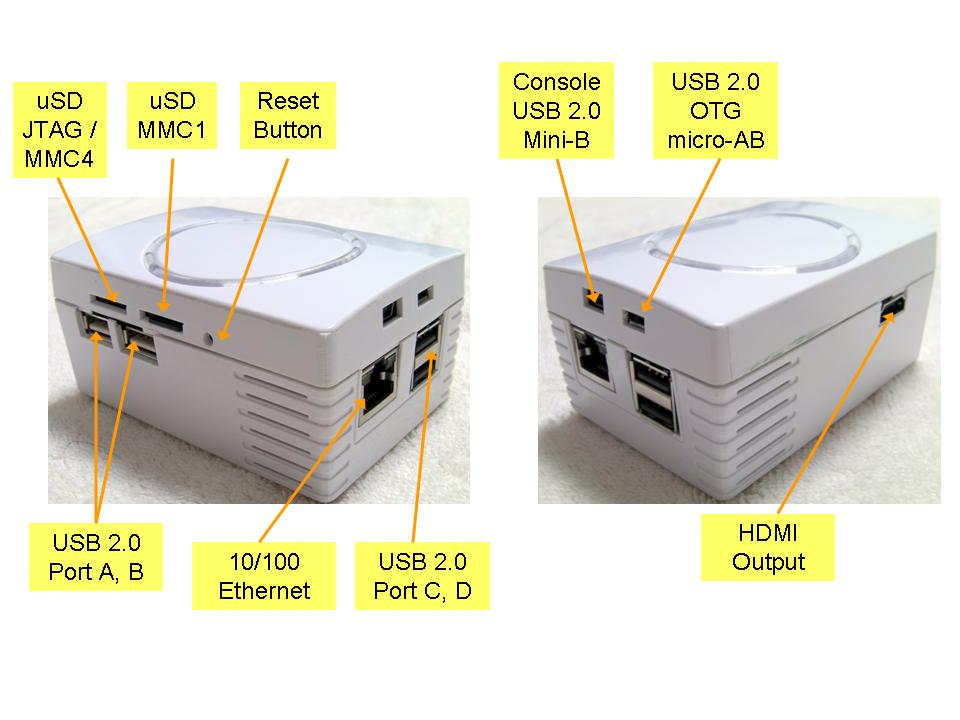
\includegraphics[width=\textwidth]{afbeeldingen/GuruPlug_Display}
	\caption{GuruPlug Display}
\end{figure}


\section{Interface module}
\label{ontwerp:hardware:interface}

De gebruikersinterface wordt gerealiseerd door 4 grote drukknoppen ingebouwd in de kast van elke kiosk. Momenteel worden deze knoppen intern doorverbonden met een afstandsbediening, waardoor de gebruiker via het indrukken van de knoppen indirect de DVD-speler kan besturen om zo een fragment te selecteren.

\begin{figure}
	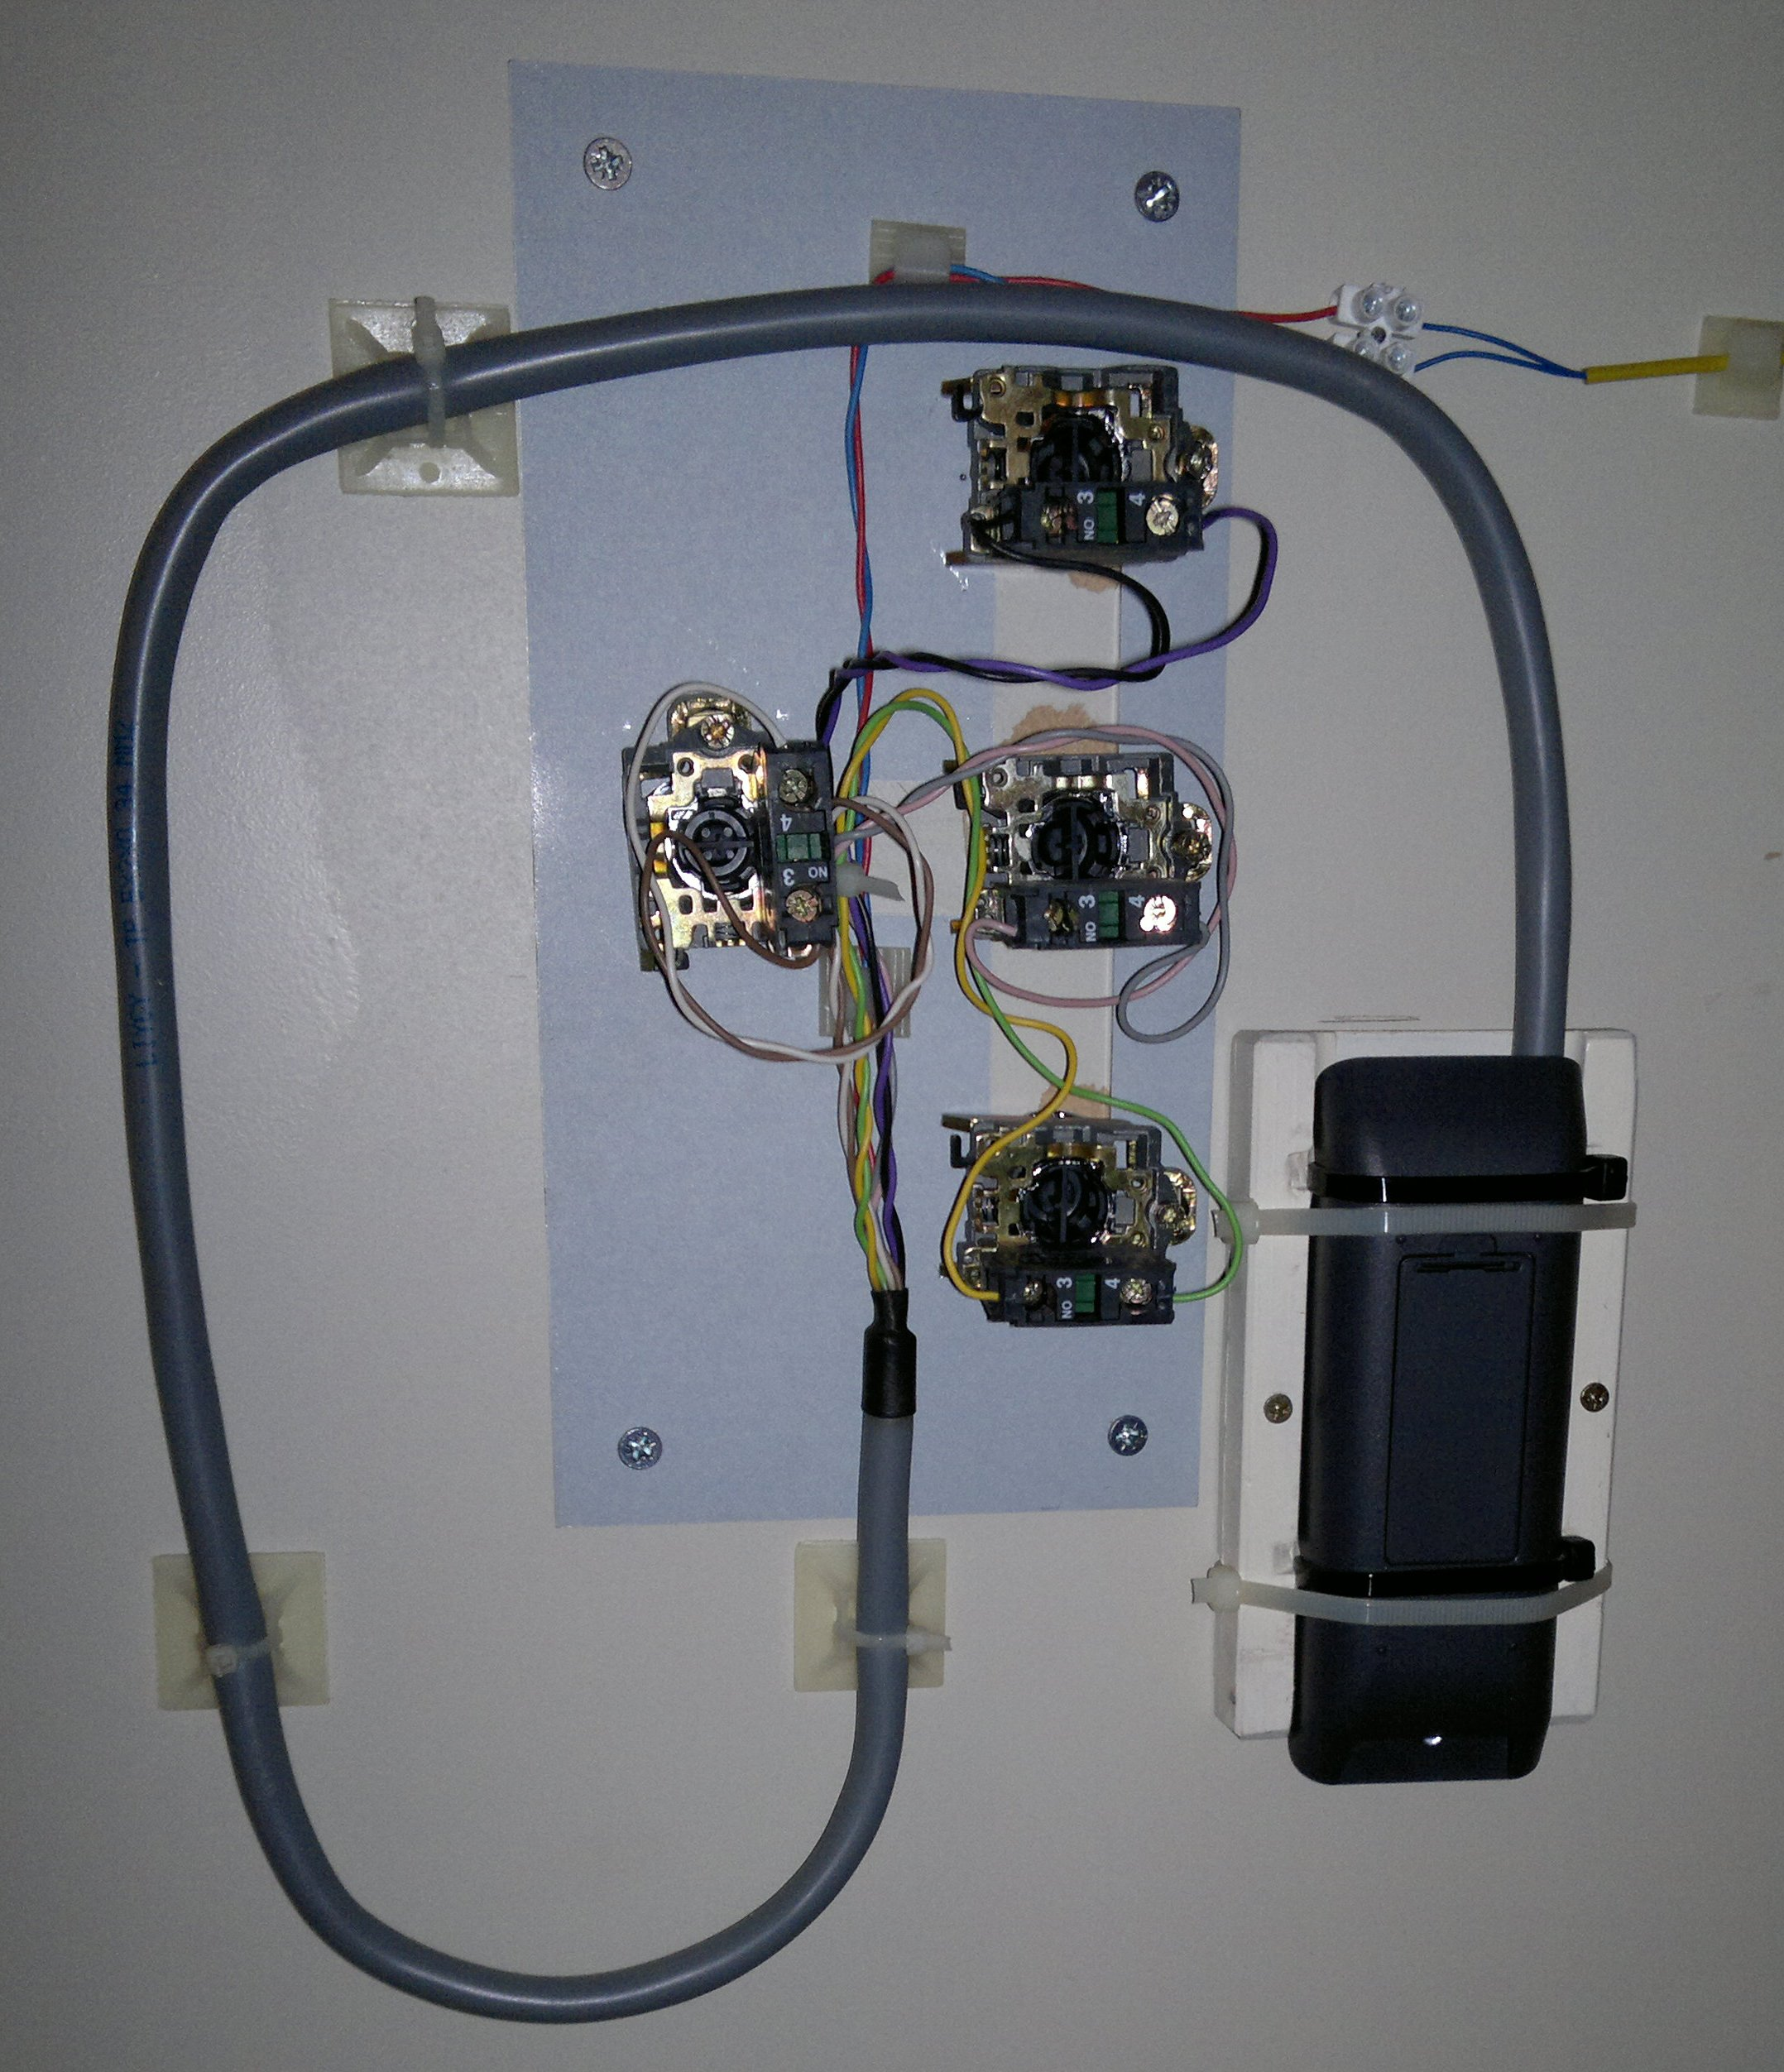
\includegraphics[width=\textwidth]{afbeeldingen/kiosk_knoppen}
	\caption{Huidige aansluitingsmethode knoppen}
\end{figure}

Nu we echter de DVD-spelers gaan vervangen door een computer, zullen we ook voor deze interface module een compatibel alternatief moeten vinden. Aan deze module worden enkele specifieke eisen gesteld:
\begin{itemize}
\item Goedkoop: de module moet zo goedkoop mogelijk te produceren zijn, alsook mag het niet teveel energie verbruiken;
\item Toekomstgericht: aansluitmogelijkheden mogen geen gebruik maken van oude protocollen;
\item Gebruiksvriendelijk: installatie van de module moet eenvoudig zijn;
\item Snel: de tijd tussen het indrukken van een toets en registratie van het signaal, moet minimaal zijn;
\item Uitbreidbaar: het moet mogelijk zijn om later extra toetsen toe te voegen aan de module.
\end{itemize}

\subsection{Aansluiting}

Het grootste ontwerpprobleem hierbij is de manier van aansluiting die we zullen gebruiken om de module in verbinding te brengen met de rest van de kioskhardware. De meeste eenvoudige keuze zou die zijn van de \strong{parallelle poort}, waarbij we de pinnen van de poort vrijwel direct zouden kunnen verbinden met de knoppen. Jammer genoeg zijn parallelle poorten steeds schaarser, en komt die vrijwel nooit meer voor op embedded hardware. Een andere toegankelijke optie is de \textbf{seriële poort}. Hierbij zou dan extra periferie benodigd zijn om in te staan voor de serializatie van de signalen, toch als we de poort op een platform-onafhankelijke manier willen uitlezen. Indien we echter platform-specifieke code toelaten, kunnen we de stuursignalen van de poort op een parallelle manier misbruiken zodat ook die periferie geëlimineerd wordt. Toch voldoet ook deze oplossing niet: ook de seriële poort wordt steeds schaarser, en alhoewel ze momenteel nog te vinden is op de meeste embedded-hardware, kan dat binnen enkele jaren het geval niet meer zijn.

Daarom hebben we uiteindelijk gekozen voor een poort die we normaal gezien wel nog enkele jaren zullen terugvinden op de meest courante hardware: de \ac{usb} poort. Deze veelzijdige poort laat ons doe om de interface module te laten communiceren met een computer, en is ook relatief toekomstgericht (de recent geïntroduceerde \ac{usb} versie 3 is nog steeds terugwaarts compatibel met \ac{usb} versie 1 toestellen). Maar het gebruik van \ac{usb} kent ook een nadeel. Het protocol is immers pakket-georiënteerd, waardoor extra periferie een noodzaak is. Ook is de configuratie complexer, zeker indien we een toestel willen dat zonder extra stuurprogramma's werkt op verschillende besturingssystemen.

\subsection{Realisatie \ac{usb}-communicatie}

Aangezien \ac{usb} een pakket-georiënteerd protocol is, hebben we steeds extra periferie nodig om de gebruikersinvoer door te sturen. Om geen speciale software te vereisen, moet onze module een apparaat uit de \ac{usb} \ac{hid} klasse implementeren. Het voordeel van deze klasse is immers dat het mogelijk is om een toestel te realiseren dat geen extra stuurprogramma's nodig heeft. Dit geldt echter enkel voor bepaalde subcategorieën van deze klasse, zoals toetsenborden, muizen, \dots Daarom zullen we onze module zichzelf laten identificeren als een toetsenbord, waarbij we dan in de Javascript code van de voorstellingen gepast kunnen reageren op dergelijke toetsaanslagen.

Om een \ac{usb} toetsenbord te realiseren, zijn we in eerste instantie op zoek gegaan naar \strong{\ac{usb} keyboard encoders}. In de huidige opzet hebben we echter maar nood aan 4 knoppen, terwijl de meeste keyboard encoders veel meer toetsen toelaten. Daarom is de prijs meestal ook een pak hoger, zo kost de \makeurl{http://www.ultimarc.com/ipacve.html}{I-Pac VE} keyboard encoder, die 32 toetsen toelaat, reeds \$35!

Daarom lijkt het interessanter om zelf te voorzien in de conversie naar \ac{usb}-pakketten, door gebruik te maken van een \strong{microcontroller met \ac{usb} hardware}. Dergelijke microcontrollers voorzien in on-chip \ac{usb} communicatiemogelijkheden, net zoals de meeste reguliere microcontrollers toelaten om gegevens over een seriële \ac{uart} te transporteren. Om vervolgens de \ac{usb} hardware op een toegankelijke manier te gebruiken, bestaan er verschillende bibliotheken zoals de officiële \ac{usb} bibliotheek van Atmel, of het open-source \makeurl{http://www.fourwalledcubicle.com/LUFA.php}{\ac{lufa}}. Het nadeel van deze piste is echter de meerkost van de \ac{usb} hardware, die eigenlijk onnodig is daar we enkel gebruik zullen maken van de \emph{low speed} overdrachtsmodus.

Een derde optie is om gebruik te maken van een \strong{microcontroller met \ac{usb} software}. Hierbij hebben we geen speciale hardware nodig, enkel een microcontroller die krachtig genoeg is om de \ac{usb} software uit te voeren. Het grote nadeel hieraan is dat het met de huidige microcontrollers enkel mogelijk is om gebruik te maken van \emph{low speed} \ac{usb}, maar voor onze toepassing is dit geen probleem. Opnieuw zijn er verschillende mogelijkheden om dit te realiseren, waaronder een \makeurl{http://www.atmel.com/dyn/resources/prod\_documents/doc2556.pdf}{application note} van Atmel. Deze application note gebruikt relatief weinig hardware om elementaire \ac{usb} communicatie te realiseren, maar zoals later zal blijken zijn er nog efficiëntere configuraties mogelijk. Ook is de software geschreven in AVR assembler, waardoor het geheel niet zo overdraagbaar is. Daarom zullen we gebruik maken van een open-source alternatief: de \makeurl{http://www.obdev.at/products/vusb/index.html}{V-USB} bibliotheek. Deze in C-geschreven bibliotheek biedt een eenvoudigere interface, alsook verschillende voorbeeldprojecten om het gebruik ervan te illustreren.